{\documentclass[11pt,a4paper,titlepage,table]{article}
\usepackage[a4paper]{geometry}
\usepackage[utf8]{inputenc}
\usepackage[english]{babel}
\usepackage{lipsum}



\usepackage{amsmath, amssymb, amsfonts, amsthm, fouriernc}
% mathtools for: Aboxed (put box on last equation in align envirenment)
\usepackage{microtype} %improves the spacing between words and letters

\usepackage{graphicx}
\graphicspath{ {./pics/} {./eps/}}
\usepackage{epsfig}
\usepackage{epstopdf}
\usepackage{colortbl}


%%%%%%%%%%%%%%%%%%%%%%%%%%%%%%%%%%%%%%%%%%%%%%%%%%
%% COLOR DEFINITIONS
%%%%%%%%%%%%%%%%%%%%%%%%%%%%%%%%%%%%%%%%%%%%%%%%%% 
\usepackage{colortbl}
\usepackage[usenames,dvipsnames,svgnames,table]{xcolor}
\usepackage{float}
%%%%%%%%%%%%%%%%%%%%%%%%%%%%%%%%%%%%%%%%%%%%%%%%%%
\definecolor{MyColor1}{HTML}{75A42E} %mix personal color
\definecolor{MyColor2}{HTML}{75A42E}
\definecolor{MyColor3}{HTML}{4D6D1E}
\definecolor{green1}{HTML}{EAF5DB}
\definecolor{green2}{HTML}{C2E193}
\definecolor{maroon}{cmyk}{0,0.87,0.68,0.32}
\newcommand{\textb}{\color{Black} \usefont{OT1}{lmss}{m}{n}}
\newcommand{\blue}{\color{MyColor1} \usefont{OT1}{lmss}{m}{n}}
\newcommand{\blueb}{\color{MyColor1} \usefont{OT1}{lmss}{b}{n}}
\newcommand{\red}{\color{LightCoral} \usefont{OT1}{lmss}{m}{n}}
\newcommand{\green}{\color{Turquoise} \usefont{OT1}{lmss}{m}{n}}
%%%%%%%%%%%%%%%%%%%%%%%%%%%%%%%%%%%%%%%%%%%%%%%%%%




%%%%%%%%%%%%%%%%%%%%%%%%%%%%%%%%%%%%%%%%%%%%%%%%%%
%% FONTS AND COLORS
%%%%%%%%%%%%%%%%%%%%%%%%%%%%%%%%%%%%%%%%%%%%%%%%%%
%    SECTIONS
%%%%%%%%%%%%%%%%%%%%%%%%%%%%%%%%%%%%%%%%%%%%%%%%%%
\usepackage{titlesec}
\usepackage{sectsty}
%%%%%%%%%%%%%%%%%%%%%%%%
%set section/subsections HEADINGS font and color
\sectionfont{\color{MyColor1}}  % sets colour of sections
\subsectionfont{\color{MyColor2}}  % sets colour of sections
\subsubsectionfont{\color{MyColor3}}  % sets colour of sections

%set section enumerator to arabic number (see footnotes markings alternatives)
\renewcommand\thesection{\arabic{section}.} %define sections numbering
\renewcommand\thesubsection{\thesection\arabic{subsection}} %subsec.num.

%define new section style
\newcommand{\mysection}{
	\titleformat{\section} [runin] {\usefont{OT1}{lmss}{b}{n}\color{MyColor1}} 
	{\thesection} {3pt} {} } 

%%%%%%%%%%%%%%%%%%%%%%%%%%%%%%%%%%%%%%%%%%%%%%%%%%
%		CAPTIONS
%%%%%%%%%%%%%%%%%%%%%%%%%%%%%%%%%%%%%%%%%%%%%%%%%%
\usepackage{caption}
\usepackage{subcaption}
%%%%%%%%%%%%%%%%%%%%%%%%
\captionsetup[figure]{labelfont={color=Turquoise}}


\makeatletter
\let\reftagform@=\tagform@
\def\tagform@#1{\maketag@@@{(\ignorespaces\textcolor{red}{#1}\unskip\@@italiccorr)}}
\renewcommand{\eqref}[1]{\textup{\reftagform@{\ref{#1}}}}
\makeatother
\usepackage{hyperref}
\hypersetup{colorlinks=true}

%%%%%%%%%%%%%%%%%%%%%%%%%%%%%%%%%%%%%%%%%%%%%%%%%%
%% PREPARE TITLE
%%%%%%%%%%%%%%%%%%%%%%%%%%%%%%%%%%%%%%%%%%%%%%%%%%
\title{\blue  
	\blueb Battle of Origins | Theory Defender}
\author{}
\date{\today}
%%%%%%%%%%%%%%%%%%%%%%%%%%%%%%%%%%%%%%%%%%%%%%%%%%



\begin{document}
	\maketitle
	\hypersetup{linkcolor=MyColor1}
	
	\begin{figure}[h!]
  		\caption{Battle of Origins | Theory Defender}
  		\centering
    	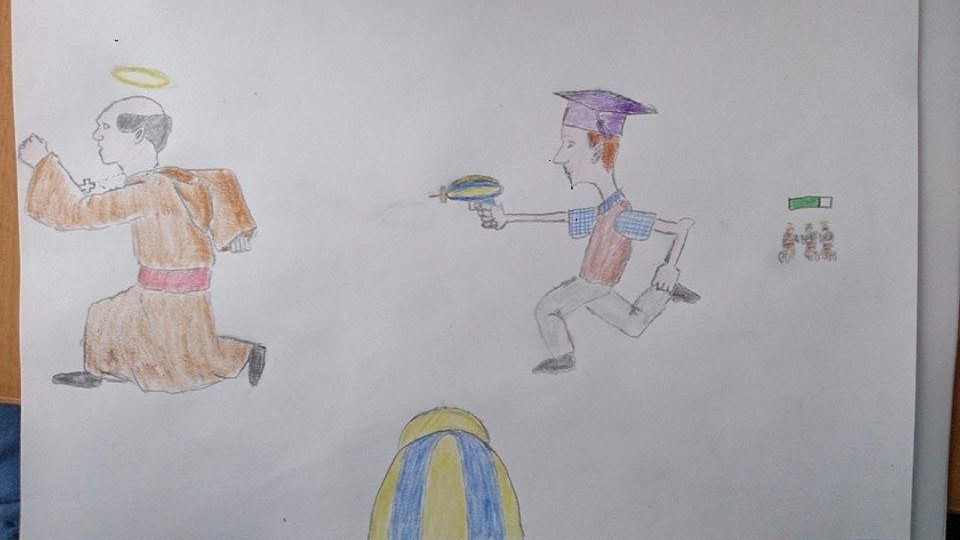
\includegraphics[width=1\textwidth]{img/FPSPerspective}
	\end{figure}	
	
	\tableofcontents
	\section{Game Description}{
		%–	 1 to 3 pages detailed description
		%–	3 pages sketches / sample images 
		%–	Highlight and justify design choices 

		\subsection{Storyline}{
			There has always been a fight going on where exactly we come from and how we got to be the way we are today. While most religions teach us that humanity was created the way we are now, evolutionists believe we have started at as a less complex species and evolved over time. Our game should settle this fight once and for all.
		}\label{sub:sub1}


		\subsection{Gameplay}{
	
			Before the match begins the player may choose a belief. Either religious or evolutionist. The main aim of the game is to convert the entire opposing team to your belief. \\
			The teams will consist of 30 people each. Non-human players will be controlled by an artificial intelligence. Each player is able to stun players of the other team making them temporarily unable to move. To convert the opposing player to your belief a big wonder must be casted. A big wonder can be generated by standing together as a group from the same team. Standing together will fill the big wonder progress bar. The speed of the progress is determined by two factors:
			\begin{enumerate}
				\item \textbf{The size of the group:}\\
							The more people close to each other, the quicker the progress bar will increase
				\item \textbf{Wonder Skill:}\\
				The creating-wonder skill of each player that is currently in the group (see subsection Evolving Upgrades)
			\end{enumerate}
			Once a big wonder is generated it is indicated by multiple visual representations:
			\begin{itemize}
				\item The progress bar is full (visible to all players)
				\item One player is now in possession of the big wonder (see subsection Visual Difference to see visual representation)
				\item A sound lets every player know that a big wonder is ready
			\end{itemize}
			The player who is in possession of the big wonder can now cast this whenever he wishes. While he is in possession he cannot be converted by a big wonder of the other team. Once the big wonder is casted, the player becomes immune to all types of attacks (main attacks, big wonder conversion) and he is able to control the big wonder's area of effect. Any opposing player who is in the area of effect will be converted to the own team.\\
			If a user controlled player is converted he takes control of another computer controlled player of the original team, as long as there still exists one. If no computer controlled player is left in the team the player enters spectator mode until computer controlled players are available again.
			
		}\label{sub:sub2}%
		%%% END SUBSECTION 2 %%%%%%%%%%%%%%%%%%%%%%%%%%%%%%%%%%%%%
		
		
		\subsubsection{Multiple Targets}
During the game the player needs to perform different tasks at the same time. On the one hand the game can only be won when a big wonder is casted and thus, players need to form study or praying groups to fill the big wonder bar. On the other hand players must prevent the other team from filling their big wonder bar. Some players in the other team will also pursue this task of distracting the prayers or the studying. Therefore, in order to win the game players also need to protect the players filling the big wonder bar.
		
		
		\subsection{Evolving Upgrades }{Players will evolve on the fly while playing. They will not have the ability to choose an upgrade themselves. The more they perform a specific action, the better they will become at it. Following is a list of automatically evolving skills:
			\begin{itemize}
				\item Running Speed
				\item Power of main attack
				\item Precision of main attack
				\item Contribution to creating a big wonder
				\item Immunity against attacks
				\end{itemize}
			The visual difference of each upgrade can be seen in subsection \ref{sec:visual_diff}
		}\label{sub:sub3}
		
		
		\subsection{Visual Difference}{
			Although each player has the same power and tools, they are visually and audibly different depending on the chosen belief. Here is a table of what each part will look like
			\subsubsection{Main Game Aspects}{ 
				See table \ref{table:main}
				\begin{table}[h!]\centering
					\begin{tabular}{r!{\color{green2}\vrule}l!{\color{green2}\vrule}l}
						& \textbf{Religious} & \textbf{Evolutionist} \\
						\rowcolor{green1}
						\textit{Main Weapon} & Insult &	Stun gun \\
						\textit{Main Weapon  (upgrade)} &	Curse&	Stun cannon \\
						\rowcolor{green1}
						\textit{Main attack}&	Curse&	Shoot stun gun/cannon  \\
						\textit{Big Wonder} & Rays of god &	Rain of books \\
						\rowcolor{green1}
						\textit{ Creating Big Wonder} &	Praying&	Studying \\
						\textit{Big Wonder finished creating sound} & Angels singing "Aaaaah" &	Pen on paper scribbling \\
						\rowcolor{green1}
						\textit{ Possessing wonder} &	Wings &	Carrying big book \\			
					\end{tabular}
				\caption*{\textit{Table \ref{table:main}: Main Game Aspects}}
				\end{table}\label{table:main}		
					
\begin{figure}[ht]
\centering
\begin{minipage}[t]{0.4\textwidth}
	\centering
	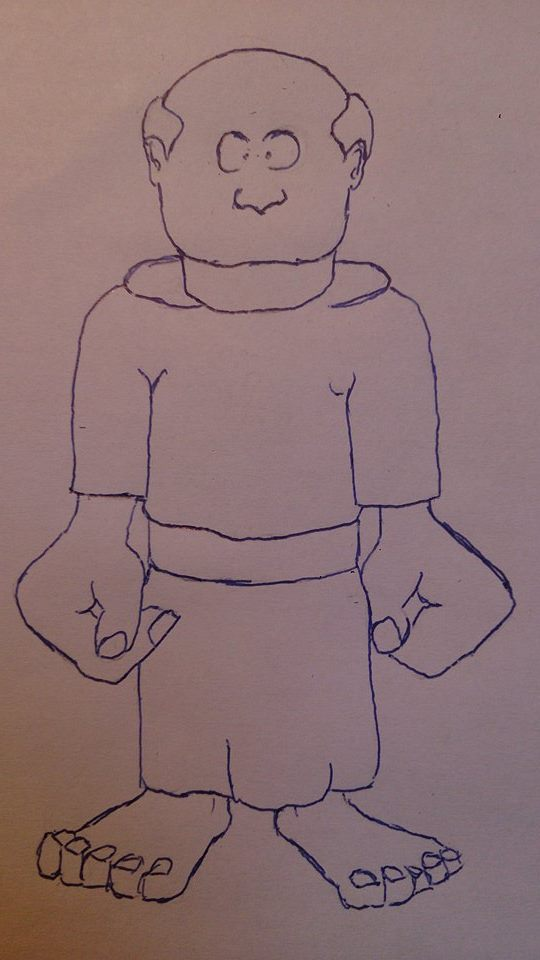
\includegraphics[width=0.7\textwidth]{img/cre-big-hands}
	\caption{Creationist}
\end{minipage}
\begin{minipage}[t]{.4\textwidth}
	\centering
	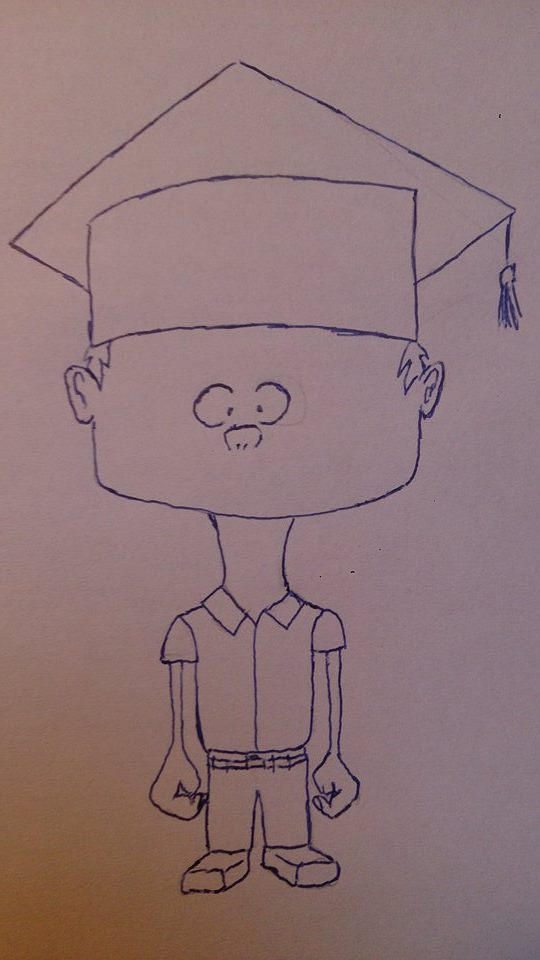
\includegraphics[width=0.7\textwidth]{img/Nerd-BigHead}
	\caption{Scientist}
\end{minipage}
\end{figure}
					
				}
				\subsubsection{Character Upgrades}{
					See table \ref{table:character}
					\begin{table}[h!]\centering
						\begin{tabular}{r!{\color{green2}\vrule}l!{\color{green2}\vrule}l}
							& \textbf{Religious} & \textbf{Evolutionist} \\
							\rowcolor{green1}
							\textit{Shoot better} & Glove color (white --> red) &	Stun gun \\
							\textit{stronger main Weapon  (upgrade)} &	Curse & Gun size (small --> big) \\
							\rowcolor{green1}
							\textit{Faster Running}&	Bigger feet &	Bigger feet  \\
							\textit{Big Wonder skill} & Size of hands (small -->  big)  &	size of head (small --> big)\\
							\rowcolor{green1}
							\textit{Immunity against attacks} &	skin color (white --> silver) & skin color (white --> silver) \\
						\end{tabular}
						\caption*{\textit{Table \ref{table:character}: Character Upgrades}}
					\end{table}\label{table:character}
						
				}
				
				\subsection{Important Aspects}{
					\begin{enumerate}
						\item \textbf{Fair Teams:}\\
							We want the teams to be equal in the sense that both possess the same offense/defense. Therefore, winning merely depends on the strategy and the aiming skills of the player
						\item \textbf{Unique Gameplay:}\\
							We want our game to be extraordinary, but still playable by common users, without directly fitting into a game category
						\item \textbf{Cartoony/Non-Photorealistic Rendering:}\\
							Since we are touching a controversial topic we blind out some seriousness by making the characters and surroundings cartoony
						\item \textbf{Visually stunning and self-explanatory:}\\
							A player should be entertained by simply watching the game. Furthermore it should be self-explanatory without the need of long tutorials
					\end{enumerate}

					
					}
		}\label{sec:visual_diff}
	
	}\label{sec:q1sec}
	
	\section{Technical Achievement}
	\label{sec:technicalachievement}
	%to be filled in
	For a game like the one presented in this document the interaction between the players is crucial. Therefore it depends a lot on a rather large group of players, such that the player won't get bored if no one else is around him to interact with. To achieve the player to feel like a part of something big, as well as being attracted by the game by lots of interactions and possibilities to behave is the balance between the board size and the number of numbers on the board.\\
	
	If the board is very large and there is only a small number of players on the field, everybody is just playing around on his own and not interaction a lot with the other players. It takes a long time to reach the other players to either attack them or to pray or study with them. An experience like this would probably not make the players to feel in love with our game immediately.\\
	
	If, on the other hand, the board is rather small and the are many players on the field, the player will feel challenged and necessary to help his team win the battle. If he has to deal with lots of enemies before being able to reach his fellow campaigners, he will stay active and motivated throughout the whole game. This is the effect we are aiming for.\\
	
	Of course it is not always possible to start a game with that many friends who can join. But since the number of players really is crucial to the game, we will provide the possibility to make use of non-player characters (\textit{NPC}), which will be controlled by the computer rather than by some human. The artificial intelligence to make these NPCs behave intelligently is the most prominent technical achievement we want to reach. For the player it should not feel different when playing with NPC or with fellow human players. Therefore the artificial intelligence should make the NPC behave similar to characters controlled by humans. On the other hand the artificial intelligence must not be too good. If an NPC is clearly better than the human player, he might feel overchallenged. Therefore we will try to find a good compromise between stupidly behaving NPCs and super-soldier NPC who are invincible.\\
	
	
	\section{"Big Idea" Bullseye}
	\label{sec:bigideabullseye}
	\textbf{Big Idea:} Don't Kill, Convert\\
	\textbf{Technical innovation:} Not a standard shooter
	%to be filled in
	
	\section{Development Schedule}{
		\subsection{Layered task breakdown}{
			\begin{enumerate}
				\item Functional Minimum 
					%Minimal items to make something you might call a game 
					\begin{itemize}
						\item Players from two teams running around
						\item Stunning each other
						\item Counting hits
					\end{itemize}
				\item Low target
				%The least possible to feel sort of “ok” about result. 
					\begin{itemize}
						\item Creating a wonder by standing together. Will convert entire team after successfully created for now.
						\item Characters visually recognizable
					\end{itemize}
				\item Desired target 
				%This is what you’re aiming for, if things go reasonably well. 
					\begin{itemize}
						\item Wonder is possessed by a player
						\item Wonder can be casted
						\item Wonder will convert other players when in area of effect
						\item Wonder visually recognizable			
					\end{itemize}
				\item High target 
				%You might get this much done if things go extremely well. 
					\begin{itemize}
						\item Other players are controlled by an advanced AI
						\item Player controls free AI when being converted
						\item Players evolves visually and numerically according to their actions
						\item Power-ups can be collected during a game session		
					\end{itemize}
				\item High target 
				%You know won’t fit into this semester, but you might add later. 
					\begin{itemize}
						\item Online multiplayer
						\item Procedural, automatic level-design (each level is different)
						\item Classes of characters (specialized for praying/studying or shooting)		
					\end{itemize}
			\end{enumerate}
		
			
			}
\subsection{Task Allocation}{
						
	See table \ref{table:taskalloc}
	
	\begin{table}[h!]\centering
		\newcounter{taskId}
		\setcounter{taskId}{0}
		\begin{tabular}{r|l|c|c|c}
			\textbf{Task} & \textbf{Description} & \textbf{Who} & \textbf{Hrs} & \textbf{Actual} \\

			\hline 
			\stepcounter{taskId} \cellcolor[gray]{0.8} & \multicolumn{4}{c}{\cellcolor[gray]{0.8} Idea Finding}\\

			\hline						
			\stepcounter{taskId}
			\thetaskId . & Brainstorming Design & All & $5$ & $7$ \\

			\hline
			\stepcounter{taskId}
			\thetaskId . & Character modelling &  & $5$ & \\
			
			\hline 
			\stepcounter{taskId} \cellcolor[gray]{0.8} & \multicolumn{4}{c}{\cellcolor[gray]{0.8} Assignments}\\
			
			\hline
			\stepcounter{taskId}
			\thetaskId . & Project Proposal Draft & All & $5$ & $5$\\
			
			\hline
			\stepcounter{taskId}
			\thetaskId . & Prototype Chapter& All & $5$ &\\						
			\hline
			\stepcounter{taskId}
			\thetaskId . & Interim Report Chapter & All & $5$ &\\
			
			\hline
			\stepcounter{taskId}
			\thetaskId . & Alpha Release Chapter & All & $5$ &\\
			
			\hline
			\stepcounter{taskId}
			\thetaskId . & Playtest Chapter & All & $5$ &\\
			
			\hline
			\stepcounter{taskId}
			\thetaskId . & Conclusion Chapter & All & $5$ &\\
			
			\hline
			\stepcounter{taskId}
			\thetaskId . & Demo Video & All & $5$ &\\
			
						\hline 
			\stepcounter{taskId} \cellcolor[gray]{0.8} & \multicolumn{4}{c}{\cellcolor[gray]{0.8} Presentation and Demos}\\
			
			\hline
			\stepcounter{taskId}
			\thetaskId . & Pitch of the Game & All & $5$ &\\
			
			\hline
			\stepcounter{taskId}
			\thetaskId . & Formal Game Proposal & All & $5$ &\\
			
			\hline
			\stepcounter{taskId}
			\thetaskId . & Paper Prototype & All & $5$ &\\
			
			\hline
			\stepcounter{taskId}
			\thetaskId . & First Playable Demo & All & $5$ &\\
			
			\hline
			\stepcounter{taskId}
			\thetaskId . & Interim Demo & All & $5$ &\\
			
			\hline
			\stepcounter{taskId}
			\thetaskId . & Alpha Release Demo & All & $5$ &\\
			
			\hline
			\stepcounter{taskId}
			\thetaskId . & Playtest presentation & All & $5$ &\\
			
			\hline
			\stepcounter{taskId}
			\thetaskId . &Final Public Presentation & All & $5$ &\\
			
			\hline 
			\stepcounter{taskId} \cellcolor[gray]{0.8} & \multicolumn{4}{c}{\cellcolor[gray]{0.8} Functional Minimum}\\
			 
			\hline
			\stepcounter{taskId}
			\thetaskId . & Physics & All & $5$ &\\	
			 
			\hline 
			\stepcounter{taskId} \cellcolor[gray]{0.8} & \multicolumn{4}{c}{\cellcolor[gray]{0.8} Low Target}\\
			 
			 \hline
			\stepcounter{taskId}
			\thetaskId . & Audio & All & $5$ & \\
			
			\hline
			\stepcounter{taskId}
			\thetaskId . & 3D character modelling & All & $10$ &  \\
			
			\hline
			\stepcounter{taskId}
			\thetaskId . & Level design (terrain and obstacles) & All & $10$ &  \\
			
			\hline 
			\stepcounter{taskId} \cellcolor[gray]{0.8} & \multicolumn{4}{c}{\cellcolor[gray]{0.8} Desired Target}\\
			 
			\hline
			\stepcounter{taskId}
			\thetaskId . & Lightning & All & $5$ &\\
			
			\hline
			\stepcounter{taskId}
			\thetaskId . & Rendering/Shaders & All & $5$ &\\
			
			\hline
			\stepcounter{taskId}
			\thetaskId . & Animation & All & $5$ &\\
			
			\hline
			\stepcounter{taskId}
			\thetaskId . & Particle Effects & All & $5$ & \\	
			
			\hline 
			\stepcounter{taskId} \cellcolor[gray]{0.8} & \multicolumn{4}{c}{\cellcolor[gray]{0.8} High Target}\\
			
			\hline
			\stepcounter{taskId}
			\thetaskId . & Artificial Intelligence & All & $5$ & \\	
			
			\hline
			\stepcounter{taskId}
			\thetaskId . & Power-ups & All & $5$ & \\
			
			\hline
			\stepcounter{taskId}
			\thetaskId . & Player evolving visually & All & $5$ & \\	
			
		\end{tabular}
		
		\caption*{\textit{Table \ref{table:taskalloc}: Task allocation}}
	\end{table} \label{table:taskalloc}			
}

						\subsection{Timeline}{
				%Detailed timeline, milestones, task accounting, deliverables
				See table \ref{table:timeline}
				
				\begin{table}[h!]\centering
					\setcounter{taskId}{0}
					\begin{tabular}{r|c|c|c|c|c|c|c|c|c|c|c}
						\textbf{Task} & \textbf{Wk1} & \textbf{Wk2} & \textbf{Wk3} & \textbf{Wk4} & \textbf{Wk5} & \textbf{Wk6} & \textbf{Wk7} & \textbf{Wk8} & \textbf{Wk9} & \textbf{Wk10} & \textbf{Wk11}      \\
						
						\hline 
			\stepcounter{taskId} \cellcolor[gray]{0.8} & \multicolumn{11}{c}{\cellcolor[gray]{0.8} Idea Finding}\\
						
						\hline						
						\stepcounter{taskId}
						\thetaskId . & & & & & & & & & & & \\
						
						\hline						
						\stepcounter{taskId}
						\thetaskId . & & & & & & & & & & & \\
						
						\hline 
			\stepcounter{taskId} \cellcolor[gray]{0.8} & \multicolumn{11}{c}{\cellcolor[gray]{0.8} Assignments}\\
						
						\hline						
						\stepcounter{taskId}
						\thetaskId . & & & & & & & & & & & \\
						
						\hline						
						\stepcounter{taskId}
						\thetaskId . & & & & & & & & & & & \\
						
						\hline						
						\stepcounter{taskId}
						\thetaskId . & & & & & & & & & & & \\
						
						\hline						
						\stepcounter{taskId}
						\thetaskId . & & & & & & & & & & & \\
						
						\hline						
						\stepcounter{taskId}
						\thetaskId . & & & & & & & & & & & \\
						
						\hline						
						\stepcounter{taskId}
						\thetaskId . & & & & & & & & & & & \\
						
						\hline						
						\stepcounter{taskId}
						\thetaskId . & & & & & & & & & & & \\
						
						\hline 
			\stepcounter{taskId} \cellcolor[gray]{0.8} & \multicolumn{11}{c}{\cellcolor[gray]{0.8} Presentation and Demos}\\
						
						\hline						
						\stepcounter{taskId}
						\thetaskId . & & & & & & & & & & & \\
						
						\hline						
						\stepcounter{taskId}
						\thetaskId . & & & & & & & & & & & \\
						
						\hline						
						\stepcounter{taskId}
						\thetaskId . & & & & & & & & & & & \\
						
						\hline						
						\stepcounter{taskId}
						\thetaskId . & & & & & & & & & & & \\
						
						\hline						
						\stepcounter{taskId}
						\thetaskId . & & & & & & & & & & & \\
						
						\hline						
						\stepcounter{taskId}
						\thetaskId . & & & & & & & & & & & \\
						
						\hline						
						\stepcounter{taskId}
						\thetaskId . & & & & & & & & & & & \\
						
						\hline						
						\stepcounter{taskId}
						\thetaskId . & & & & & & & & & & & \\
						
						\hline 
			\stepcounter{taskId} \cellcolor[gray]{0.8} & \multicolumn{11}{c}{\cellcolor[gray]{0.8} Functional Minimum}\\
						
												\hline						
						\stepcounter{taskId}
						\thetaskId . & & & & & & & & & & & \\
						
						\hline 
			\stepcounter{taskId} \cellcolor[gray]{0.8} & \multicolumn{11}{c}{\cellcolor[gray]{0.8}Low Target}\\
						
						\hline						
						\stepcounter{taskId}
						\thetaskId . & & & & & & & & & & & \\
						
						\hline						
						\stepcounter{taskId}
						\thetaskId . & & & & & & & & & & & \\
						
						\hline						
						\stepcounter{taskId}
						\thetaskId . & & & & & & & & & & & \\
						
						\hline 
			\stepcounter{taskId} \cellcolor[gray]{0.8} & \multicolumn{11}{c}{\cellcolor[gray]{0.8} Desired Target}\\
						
						\hline						
						\stepcounter{taskId}
						\thetaskId . & & & & & & & & & & & \\
						
						\hline						
						\stepcounter{taskId}
						\thetaskId . & & & & & & & & & & & \\
						
						\hline						
						\stepcounter{taskId}
						\thetaskId . & & & & & & & & & & & \\
						
						\hline						
						\stepcounter{taskId}
						\thetaskId . & & & & & & & & & & & \\
						
						\hline 
			\stepcounter{taskId} \cellcolor[gray]{0.8} & \multicolumn{11}{c}{\cellcolor[gray]{0.8} High Target}\\
						
						\hline						
						\stepcounter{taskId}
						\thetaskId . & & & & & & & & & & & \\
						
						\hline						
						\stepcounter{taskId}
						\thetaskId . & & & & & & & & & & & \\
						
						\hline						
						\stepcounter{taskId}
						\thetaskId . & & & & & & & & & & & \\
								
					\end{tabular}
					
					\caption*{\textit{Table \ref{table:timeline}: Timeline\\ A = All, P = Patrick, R = Ruben, J = Jacqueline, G = Gregory}}
				\end{table} \label{table:timeline}
			
			
				
				
		\section{Assessment}{
			%Strengths, appeal, criteria for success…
			Our game shall stand out in several ways. We want to create a funny, cartoony, visual stunning gaming experience that fascinates someone by only watching another person playing the game. By “funny” we mean that everything from design over physics to sound will be produced with always keeping humour at the back of one’s mind. For example, if a character gets hit by an enemy’s shot, it will fly through the air far away from real-world physics. Also, we want to include a dimension of “cuteness” into our gaming experience by using non-photorealistic rendering and a cartoony overall look. We believe that the combination of cartoony visuals, a camera that shows a wide part of the action and a fast effect-overloaded gameplay will create a special form of appealing that will bring the player in a good mood and provides an experience of fun in every second of playing. By “visual stunning” we want to say that the player will see a battlefield with a lot of characters fighting each other and building pray/study circles, objects that are hit and therefore flying through the air, different looking characters according to their skills and a lot of light and particle effects caused by the weapons, power-ups or the skills of characters.
			As criteria for success we elaborated our own “big idea bullseye”. On the one hand, our core idea consists of the effect-overloaded non-realistic cartoony styled fight over evolution including the “super-power” of converting enemies. On the other hand, our technical innovation is a shooter where you can’t kill enemies and where team play is crucial to win the game.
			
		}
	}	
	
\end{document}}{den}